\chapter{Konzeption}

\section{MEMA-Prinzip}
Die des MEMA-Prinzip findet sich in der Diplomarbeit von Timo-Weithöhner. Es ermöglicht die Abspeicherung einer Ontolgie in eine Datenbank mit einem festen Satz von Tabellen. Dies vereinfacht es Regeln in SQL zu erstellen, da diese vorformuliert werden können.

Das ursprüngliche MEMA-Prinzip von Timo Weithöhner ist um folgende Punkte erweitert.
Es wurde erstmal auf den erweiterten Sprachschatz von OWL2 RL angepasst. Was aber besonders zu erwähnen ist sind die Relationen list und history. Sie speichern keine Axiome wie alle anderen. list dient als Hilfstruktur für Axiome die eine variable Anzahl von Elementen abspeichern. history wird benutzt, um benutzt um den Abhängigkeitsverlauf beim inferieren von von Fakten speichern zu können. Damit ist es möglich Ableitungen gezielt wieder rückgängig zu machen. Deswegen sind auch alle anderen Relationen mit einer id Spalte ausgestattet, die Axiome eindeutig identifiziert.

Allgemein wurd bei der Erstellung der Tabellenstruktur darauf geachtet, das die Formulierung der Regeln in SQL vereinfacht wird. So ist im Normalfall die Ergebnismenge einer Regel dadurch zu erhalten, in dem man die beteiligten Relationen miteinander joinet auf den Variablen, die in den Regeln angegeben sind.

Abbildung der Tabellenstruktur im Anhang
\tikzstyle{relation}=[rectangle, draw=black, rounded corners, fill=white, drop shadow, text justified, anchor=north, text=black, text width=4cm]

\begin{tikzpicture}[node distance=6cm]
	\node (history) [relation, rectangle split, rectangle split parts=2]{
			\textbf{history}
		\nodepart{second}
			\underline{id}: INT\newline
			\underline{table}: TABLE\newline
			\underline{sourceId}: INT\newline
			\underline{sourceTable}: TABLE
	};
	\node (list) [relation, rectangle split, rectangle split parts=2, left of= history]{
			\textbf{list}
		\nodepart{second}
			id: INT\newline
			\textbf{\underline{name}}: CLASS\newline
			\textbf{\underline{element}}: CLASS/IND
	};

\end{tikzpicture}


\tikzstyle{relation}=[rectangle, draw=black, rounded corners, fill=white, drop shadow, text justified, anchor=north, text=black, text width=5cm]
\begin{tikzpicture}[node distance=3cm]
	\node (subClass) [relation, rectangle split, rectangle split parts=2]{
			\textbf{subClass}
		\nodepart{second}
			\underline{id}: INT\newline
			\textbf{\underline{sub}}: CLASS\newline
			\textbf{\underline{super}}: CLASS
	};
	
	
	\node (classAssertionEnt) [relation, rectangle split, rectangle split parts=2, below of= subClass]{
			\textbf{classAssertionEnt}
		\nodepart{second}
			\underline{id}: INT\newline
			\textbf{\underline{entity}}: IND/CLASS\newline
			\textbf{\underline{class}}: CLASS
	};
	
	\node (classAssertionLit) [relation, rectangle split, rectangle split parts=2, right =2cm of classAssertionEnt]{
			\textbf{classAssertionLit}
		\nodepart{second}
			\underline{id}: INT\newline
			\textbf{\underline{literal}}: IND/CLASS\newline
			\textbf{\underline{class}}: CLASS\newline
			\textbf{\underline{language}}: LANGUAGE
	};
	
	\node (sameAsEnt) [relation, rectangle split, rectangle split parts=2, below =2cm of classAssertionEnt]{
			\textbf{sameAsEnt}
		\nodepart{second}
			\underline{id}: INT\newline
			\textbf{\underline{left}}: IND\newline
			\textbf{\underline{right}}: IND
	};
	
	\node (sameAsLit) [relation, rectangle split, rectangle split parts=2, right =2cm of sameAsEnt, text width=6cm]{
			\textbf{sameAsLit}
		\nodepart{second}
			\underline{id}: INT\newline
			\textbf{\underline{left}}: IND\newline
			\textbf{\underline{right}}: IND\newline
			\textbf{\underline{left\_type}}: CLASS\newline
			\textbf{\underline{right\_type}}: CLASS\newline
			\textbf{\underline{left\_language}}: LANGUAGE\newline
			\textbf{\underline{right\_language}}: LANGUAGE
	};
	
	\node (objectPropertyAssertion) [relation, rectangle split, rectangle split parts=2, below =2cm of sameAsEnt]{
			\textbf{objectPropertyAssertion}
		\nodepart{second}
			\underline{id}: INT\newline
			\textbf{\underline{subject}}: IND\newline
			\textbf{\underline{property}}: PROPERTY\newline
			\textbf{\underline{object}}: IND
	};
	
	\node (dataPropertyAssertion) [relation, rectangle split, rectangle split parts=2, right =2cm of objectPropertyAssertion, text width=6cm]{
			\textbf{dataPropertyAssertion}
		\nodepart{second}
			\underline{id}: INT\newline
			\textbf{\underline{subject}}: IND\newline
			\textbf{\underline{property}}: PROPERTY\newline
			\textbf{\underline{object}}: LITERAL\newline
			\textbf{\underline{type}}: CLASS\newline
			\textbf{\underline{language}}: LANGUAGE
	};

\end{tikzpicture}


\section{Arbeitsablauf des Schlussfolgerers}
Alle Axiome werden entsprechend dem MEMA-Prinzip abgelegt. Dabei ist für jedes Axiom genau eine Relation vorgesehen. Für gewisse Axiome werden implizite Informationen abgelegt, wie. z.B.

ObjectProperty Assertion a p n --> p type ObjectProperty

Falls ein Axiom aus komplexen Ausdrücken zusammengesetzt ist werden die Ausdrücke rekursiv abgearbeitet und einzeln behandelt. Zum herstellen der Beziehungen beim komplexen Axiomen werden Platzhalter für die Ausdrücke verwendet. Die Platzhalter die dabei erzeugt werden stammen von der OWLAPI aus der NodeID Klasse und folgen damit dem selben Schema wie auch bei anonymen Individuen.

Bsp:

(A int (Svf p B)) subC C
      nid1             C    subClass(nid1, C)
      nic2                  intOf(nid1, nid2)
 A         nid3             list(nid2, A, nid3)
            p B             svf(nid3, p, B)


Wenn Fakten in eine Relation geschrieben werden, wird von dieser ein Hinweis (Reason) an den Regelprozessor geschickt.

Dieser überprüft die Ursache und legt entsprechende Regeln an, die auf diese Veränderung ausgeführt werden können.

Die abzarbeitenden Regeln enthalten eine Referenz auf die Fakten, die hinzugekommen sind. Allgemein sind sie so implementiert, das sie nur auf diesen neuen Fakten arbeiten -  auf den sogenannten Deltas - dies ist allerdings nicht in allen Fällen möglich (cls-int1), sinnvoll (zu viele verschiedene Kombinationsmöglichkeiten) oder einfach zu komplex und damit fehleranfällig (prp-spo2). Falls zwei oder mehrmals eine Regel auf die selben neuen Fakten erzeugt wird bevor sie ausgelöst wird, werden die beiden Regeln zu einer zusammengefasst und können je nach Einstellung neu priorisiert werden.
--------
Durch eine spezielles Priorisierungsverfahren wäre es evtl. möglich zielgerichtet auf die Erzeugung gewisser Fakten hinzuarbeiten.

Was sind Fakten?

Was ist eine Ontologie?

Was sind Deltas?

Was ist eine Relation?
--------
All diese Regeln sind in einer Warteschleife abgelegt, die beim laden der Ontologie gefüllt wird und beim ab arbeiten, d.h. dem realisieren, der Ontologie ausgelesen wird.

Regeln können durch das Erzeugen von neuen Fakten Hinweise für an den Regelprozessor geben der daraufhin weiter Regeln anlegt und in die Warteschlange einsortiert.

Der Vorgang des realisierens ist abgeschlossen, wenn keine Regel neue Fakten und damit neue Regeln erzeugen kann.

Der OWL2 RL Regelsatz garantiert dabei, das es immer zu einem Ende der Regelanwendung kommen wird, egal ob eine gültige oder ungültige Ontologie geladen wird.

Für das Abarbeiten und Erzeugen der Regeln ist hauptsächlich der Regelprozessor verantwortlich. Hier sind noch weitere Einstellungsmöglichkeiten, wie z.B. die parallele Verarbeitung von Regeln vorhanden.

Nachfolgend eine Übersicht über einen Ablauf des Schlussfolgerers, wenn er eine neue Ontologie lädt (Standardfall).

\begin{figure}
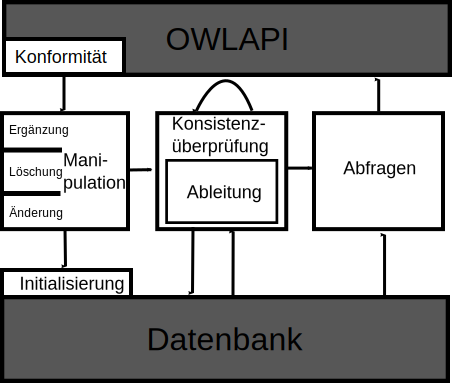
\includegraphics{images/u2r3-workflow.pdf}
\end{figure}


Speicherung

In welcher Struktur die Ontolgie in der Datenbank abgelegt wird, wurde bereits mit dem MEMA-Prinzip erklärt. Es lässt eine Speicherung zu, die sehr nach an den Axiomen aber auch den Regeln liegt und damit eine effiziente und angenehme Umsetzung der Regeln ermöglicht. Das ursprüngliche MEMA-Prinzip wurde dabei auf OWL2 angepasst und eine Möglichkeit zur Abspeicherung der Löschhierarchie erweitert. Diese ermöglicht es Schlussfolgerungen wieder gezielt rückgängig zu machen.

OWLAPI Anbindung

Der obere Teil ist die sogenannte OWLAPI. Die OWLAPI ist eine Bibliothek die das Auslesen von Ontologien in verschiedenen Formaten erlaubt und eine Schlussfolgererschnittstelle für andere Programme zur Verfügung stellt. Durch die Implementierung dieser Schnittstelle in U2R3 ist es für alle Programme zugänglich die mit der OWLAPI arbeiten.
Die Schnittstelle stellt dabei auch eine Liste typischer Abfragen für einen Reasoner dar und kann allein dadurch schon als Messlatte für die Fähigkeiten eines Schlussfolgerers verwendet werden. Das OWLAPI-Projekt ist open-source und in Java implementiert und ist damit auch optimal für die Implementierung von U2R3 geeignet. Neben der reinen Parsertätigkeit kann die OWLAPI auch noch helfen zu überprüfen, ob eine Ontologie im OWL2 RL Profil liegt und nimmt damit weitere Arbeit ab.



\section{Aufbau des Schlussfolgerers}



\tikzstyle{composition}=[->, >=diamond, thick]

\tikzstyle{class}=[rectangle, draw=black, rounded corners, fill=white, drop shadow, text centered, anchor=north, text width=3.5cm, rectangle split, rectangle split parts=1]

\begin{tikzpicture}[node distance=2cm]
    \node (U2R3Reasoner) [class]
        {
            \textbf{U2R3Reasoner}
%            \nodepart{second}name
        };
        
    \node (RuleManager) [class, below of= U2R3Reasoner]
        {
            \textbf{RuleManager}
%            \nodepart{second}name
        };
        
     \node (RelationManager) [class, left =0.1cm of RuleManager]
        {
            \textbf{RelationManager}
%            \nodepart{second}name
        };
        
    \node (ReasonProcessor) [class, rectangle split parts=2, right =0.1cm of RuleManager]
        {
            \textbf{ReasonProcessor}
            \nodepart{second}+ classify()
        };
        
    \draw[composition] (RuleManager.north) -- (U2R3Reasoner.south);
    \draw[composition] (RelationManager.north) -- (U2R3Reasoner.south);
    \draw[composition] (ReasonProcessor.north) -- (U2R3Reasoner.south);
        
        
\end{tikzpicture}
        

\section{Auswertungsstrategien}
Modusname: '''!EvaluationStrategy''' := COMMONLAST | RARELAST

== Alle Regeln nacheinander ==
trivial (nicht implementiert, sollte in der !RuleActionQueue umgesetzt werden)

== Abhängigkeiten der Regeln ausnutzen/Regeln in eine Queue packen ==

Regeln zusammenfassen, falls sie mehrmals angefragt werden

 * an ihrer Position in der Queue lassen
 * zurückschieben '''im Moment implementiert''' (siehe !RuleActionQueue)

== Regelauslösung ==
Für jeden Manipulation der Datenbank (DELETE/INSERT) wird/muss eine Reason ausgelöst (werden). Es wird dabei nur eine Reason ausgelöst, egal wieviele Zeilen von der Manipulation betroffen war. Eine Reason löst dann weitere Actions aus, je nachdem welche Regeln davon betroffen sind.


%{{{
DB Manipulation  (1) ===> (1) Reason (1) ===> (n) RuleActions
%}}}

%{{{
           Realtion                     Delta
%            ######
%            ######         <===           #
%            ######
                                          |
(welche Regel) |                          | (welche neuen Daten)
               |                          |
%                ####>  Reason  <==========

                          | (1)
                          |
                          | (eine Regel mit neuen Daten)
                          |
                          v (n)

                      RuleAction

%}}}

\subsubsection{Komplexe Ausdrücke finden}
\begin{verbatim}
Was sind komplexe Ausdrücke?
\end{verbatim}


Einfügen von Statements oder Werten nicht gut, weil darüber nicht geschloßen werden kann bzw. wenn darüber Aussagen gemacht werden sollen muss erst geschloßen werden. Das ist allerdings immer sehr zeitaufwendig.

\begin{verbatim}
    * Was ist der Unterschied zu OWL1 DL/Lite?
    * Was sind Fähigkeiten, die der neue U2R2 haben soll?
          o Schlussfolgern, Konsistenzprüfung, Änderung, Löschung, OWLAPI Anbindung, Konformitätsüberprüfung auf OWL2 RL 
    * Wie konform und semantisch korrekt war U2R2?
    * Was ist der Unterschied in der Menge und Art der Regelimplementierung
          o Welche Techniken wurden verwendet
          o Wieviele wurden implementiert
                + Aussagekraft der Sprachen 
          o Wie komplex sind die implementierten Regeln? Wären alle Regeln aus u2r3 auch in u2r3 implementierbar gewesen, oder wie aufwändig wäre es gewesen diese zu implementieren?
                + Lohnt sich deshalb schon der Umstieg auf ein RDBMS? (einfachere Aufbau, standardisierte Funktionen, größere Funktionsumfang) 
    * Wie wird die Trennung von Klassen und Individuen im MEMA-Modell erhalten?
    
    
        * Welche Fragestellungen gibt es?
    * Wie hängen diese zusammen?
    * Wie können spätere Manipluationen durchgeführt werden?
    * Was ist der Aufwand nach einer Änderung (von Fakten oder Konzepten)?
    * Was ist die Ausdrucksmächtigkeit von OWL2 RL?
    * Was ist die Zeit und Speicher Komplexität von OWL2 RL?
    * Was ist der Unterschied zur Ausdrucksmächtigkeit von U2R2 (1)?
    * Welche Erkenntisse gibt es bereits?
    * Was sind die Fähigkeiten/Ausdrucksmächtigkeiten der verschiedenen Fragmente?
    * Was sind ihre Komplexitäten?
    * Was versteht man unter Truth-Maintenance? 


    * Wie muss dadurch über die entstandenen Daten geschloßen werden?
    * Was sind deduktive Datenbanken?
    * Können die SQL Statements generiert werden?
    * Wie bildet man Regeln allgemein auf SQL ab? RAP?
    * Kann man quadrat. Rekursion im auflösen?
    * Wie sieht das DB-Schema aus?
    * Kann man manche Ableitungsschritte zusammenfassen?
    * Was bringen rekursive Abfragen wirklich? (Es werden dadurch ja auch andere Regeln angestoßen und dann müssen die rekursiven wieder ran)
    * Wie wandelt man die Ontologie in INSERTs um? 
\end{verbatim}



    
     